\documentclass{beamer}
\usepackage[utf8x]{inputenc}
\usepackage{hyperref}
\usepackage[footheight=1em]{beamerthemeboxes}
\usepackage{listings}
\usepackage{color}
%\usepackage{pgfpages}
%\setbeameroption{show notes on second screen=left}
\usetheme{Singapore}

%\usetheme{Frankfurt}


%\addfootboxtemplate{\color{white}}{\color{gray}
  %\insertframenumber/\inserttotalframenumber\null}



\setbeamertemplate{background canvas}{\includegraphics
   [width=\paperwidth,height=\paperheight]{files/fond.png}}


\title{Thésaurus Rex}
\author{Baptiste \textsc{Le-Bail} \and Thibaut \textsc{Marmin} \\ Namrata \textsc{Patel} \and Clément \textsc{Sipieter} \\ Steeve \textsc{Tuvée}}
\institute{Projet BDD GMIN103 : réalisation d'un Thésaurus\\\texttt{https://github.com/thibautmarmin/bdd\_projet/}}
\date{20 Janvier 2012}

\begin{document}

% Def variable coloration code source
\definecolor{keyword}{rgb}{0.55,0,0} 
\definecolor{type}{rgb}{0,0.55,0} 
\definecolor{comment}{rgb}{0.7,0.7,0.7} 

\lstset{
basicstyle=\footnotesize\sffamily,
numbers=none,
numberstyle=\footnotesize\color{comment},
keywordstyle=\color{keyword}\bfseries,
commentstyle=\color{comment},
breaklines=true,
fontadjust=true,
columns=fullflexible,
morekeywords=true
}

\AtBeginSection[]
{
  \begin{frame}{Thésaurus Rex}
  \begin{columns}[t]
  \begin{column}{5cm}
  \tableofcontents[sections={1-3},currentsection,hideothersubsections]
  \end{column}
  \begin{column}{5cm}
  \tableofcontents[sections={4-6},currentsection,hideothersubsections]
  \end{column}
  \end{columns}
  \end{frame}
}

\begin{frame}
\titlepage
\end{frame}

\begin{frame}{Thésaurus Rex}
    

  \begin{columns}[t]
  \begin{column}{5cm}
  \tableofcontents[sections={1-3},hideallsubsections]
  \end{column}
  \begin{column}{5cm}
  \tableofcontents[sections={4-6},hideallsubsections]
  \end{column}
  \end{columns}

\end{frame}

\section{Besoins}
\subsection{Fonctionnalités}
\begin{frame}{Fonctionnalités}{Diagramme de cas d'utilisations}
\begin{center}
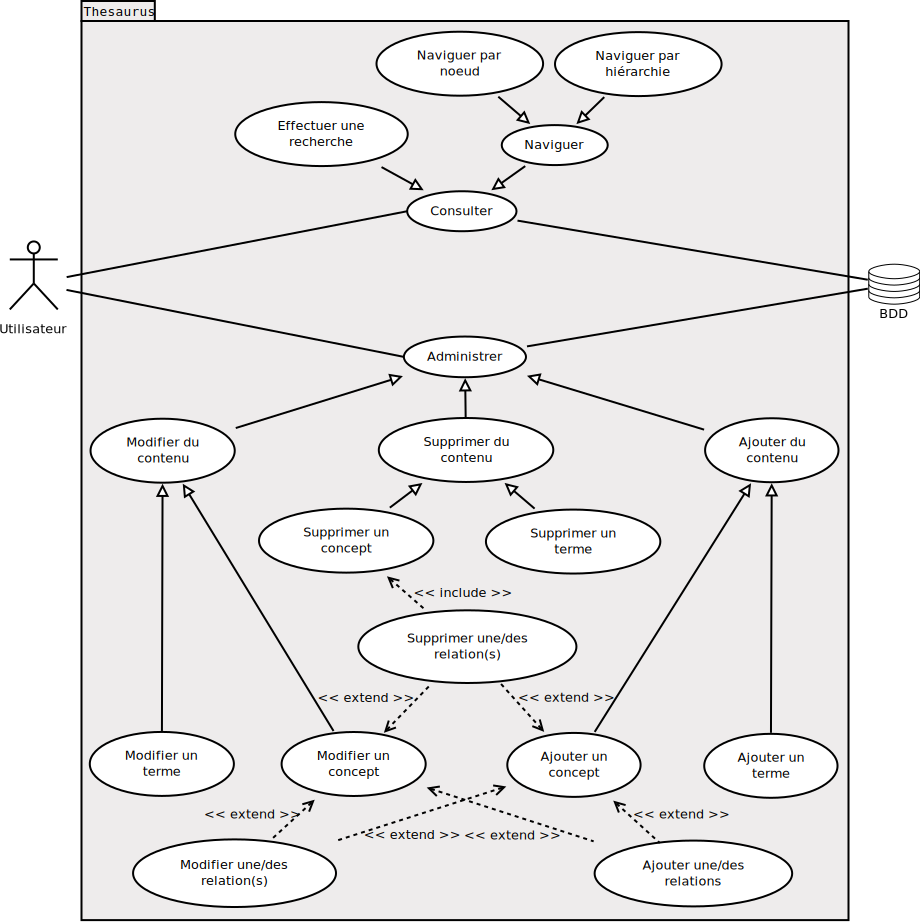
\includegraphics[width=0.6\textwidth]{files/usecase}
\end{center}
\end{frame}


\section{Modélisation}
\begin{frame}{Modélisation}
	Deux type d'entités :
	\begin{itemize}
	\item Termes
	\item Concepts
	\end{itemize}
\end{frame}

\subsection{Une première piste}
\begin{frame}{Une première piste}{Diagramme de classes}
\begin{center}
\includegraphics[width=0.5\textwidth]{files/class_v1}
\end{center}
\end{frame}

\subsection{Évolution}
\begin{frame}{Évolution}{Diagramme de classes}
\begin{center}
\includegraphics[width=0.5\textwidth]{files/class_v2}
\end{center}
\end{frame}

\subsection{Décision finale}
\begin{frame}{Décision finale}{Diagramme de classes}
\begin{center}
\includegraphics[width=0.6\textwidth]{files/class_v3}
\end{center}
\end{frame}


\section{Choix de conception}
\subsection{Paradigmes}
\begin{frame}{Paradigmes}{Vision objet}
(+ et -)
\end{frame}

\begin{frame}{Paradigmes}{Vision objet-relationnel}
(+ et -)
\end{frame}

\begin{frame}{Paradigmes}{Vision relationnel pur}
(+ et -)
\end{frame}

\subsection{ORM}
\begin{frame}{ORM}{Qu'est ce qu'un ORM ?}
\end{frame}

\begin{frame}{ORM}{Pourquoi ?}
\end{frame}

\subsection{Décision}
\begin{frame}{Décision}
\end{frame}

\section{Implémentation}
\subsection{Framework}
\begin{frame}{Framework}{Symfony2}



\begin{columns}[t]
  \begin{column}[l]{0.5\textwidth}
		\begin{block}{Histoire}
			\begin{itemize}
				\item Créé en 1998
				\item SensioLabs
				\item Framework aujourd'hui mature
			\end{itemize}
		\end{block}
	\end{column}
    \begin{column}[l]{0.5\textwidth}
		\begin{block}{Caractéristiques}
			\begin{itemize}
				\item MVC (Mojavi)
				\item ORM (Doctrine2)
				\item Template (Twig)
			\end{itemize}
		\end{block}
	\end{column}
\end{columns}
\end{frame}

\begin{frame}{Framework}{Structure des applications}
\begin{columns}[t]
    \begin{column}[l]{0.5\textwidth}
		\begin{block}{Bundle}
			\begin{itemize}
				\item module ou plugin
				\item portable
				\item facilement installable
				\item architecture MVC
			\end{itemize}
		\end{block}
	\end{column}
    \begin{column}[l]{0.5\textwidth}
		\begin{block}{Entity}
			\begin{itemize}
				\item classe
				\item paramétrable avec l'ORM
				\item contrôleur
				\item formulaires
			\end{itemize}
		\end{block}
	\end{column}
\end{columns}
\end{frame}

\begin{frame}{Framework}{ORM Doctrine2}
\begin{block}{Doctrine2}
\begin{itemize}
\item ORM populaire
\item GNU LGPL
\end{itemize}
\end{block}

\begin{block}{Intégration}
\begin{itemize}
\item ORM par défaut de Symfony
\item tag \texttt{@ORM}
\end{itemize}
\end{block}
\end{frame}

\subsection{Structure de l'application}
\begin{frame}{Structure}{Entité \emph{Terme}}
\lstinputlisting[language=PHP,morekeywords={class, public, function, return, private, namespace, use,as}]{./sources/Terme1.php}
\end{frame}

\begin{frame}{Structure}{Entité \emph{Terme}}
\lstinputlisting[language=PHP,morekeywords={class, public, function, return, private, namespace, use,as}]{./sources/Terme2.php}
\end{frame}

\begin{frame}{Structure}{Entité \emph{Concept}}
\lstinputlisting[language=PHP,morekeywords={class, public, function, return, private, namespace, use,as}]{./sources/Concept1.php}
\end{frame}

\begin{frame}{Structure}{Entité \emph{Concept}}
\lstinputlisting[language=PHP,morekeywords={class, public, function, return, private, namespace, use,as}]{./sources/Concept2.php}
\end{frame}

\begin{frame}{Structure}{Entité \emph{Concept}}
\lstinputlisting[language=PHP,morekeywords={class, public, function, return, private, namespace, use,as}]{./sources/Concept3.php}
\end{frame}

\begin{frame}{Structure}{Entité \emph{Concept}}
\lstinputlisting[language=PHP,morekeywords={class, public, function, return, private, namespace, use,as}]{./sources/Concept4.php}
\end{frame}

\begin{frame}{Structure}{Entité \emph{Concept}}
\lstinputlisting[language=PHP,morekeywords={class, public, function, return, private, namespace, use,as}]{./sources/Concept5.php}
\end{frame}

\begin{frame}{Structure}{Entité \emph{Concept}}
\lstinputlisting[language=PHP,morekeywords={class, public, function, return, private, namespace, use,as}]{./sources/Concept6.php}
\end{frame}

\subsection{Schéma relationnel généré}
\begin{frame}{Schéma relationnel généré}
\begin{description}
\item[terme](\underline{id})
\item[concept](\underline{id}, terme\_vedette\_id$^\#$, concept\_general\_id$^\#$)
\item[concept\_terme](\underline{concept\_id$^\#$, terme\_id$^\#$})
\item[concept\_concept](\underline{concept1\_id$^\#$, concept2\_id$^\#$})
\end{description}
\end{frame}

\subsection{Templates finaux}
\begin{frame}{Templates finaux}{Accueil}
\begin{center}
\includegraphics[width=\textwidth]{files/screen_accueil}
\end{center}
\end{frame}

\begin{frame}{Templates finaux}{Liste des concepts}
\begin{center}
\includegraphics[width=\textwidth]{files/screen_concepts}
\end{center}
\end{frame}

\begin{frame}{Templates finaux}{Environnement sémantique direct}
\begin{center}
\includegraphics[width=\textwidth]{files/screen_concept}
\end{center}
\end{frame}

\begin{frame}{Templates finaux}{Ajout / Modification d'un concept}
\begin{center}
\includegraphics[width=\textwidth]{files/screen_concept_edit}
\end{center}
\end{frame}

\begin{frame}{Templates finaux}{Liste des termes}
\begin{center}
\includegraphics[width=\textwidth]{files/screen_termes}
\end{center}
\end{frame}

\begin{frame}{Templates finaux}{Modification d'un terme}
\begin{center}
\includegraphics[width=\textwidth]{files/screen_terme_edit}
\end{center}
\end{frame}

\section{Conclusion \& Démonstration}
\begin{frame}{Conclusion \& Démonstration}
\end{frame}

\end{document}